\documentclass[12pt]{article}
\usepackage{graphicx}
\usepackage{amssymb}
\usepackage{epstopdf}
\usepackage{amsmath}
\usepackage{multicol}
\usepackage{tcolorbox}
\usepackage{geometry}
\usepackage{enumitem}
\usepackage{fancyhdr}

\DeclareGraphicsRule{.tif}{png}{.png}{`convert #1 `dirname #1`/`basename #1 .tif`.png}

\textwidth = 6.5 in
\textheight = 9 in
\oddsidemargin = 0.0 in
\evensidemargin = 0.0 in
\topmargin = -23pt
\headheight = 0.0 in
\headsep = 0.0 in
\parskip = 0.2in
\parindent = 0.0in
\pagestyle{fancy}
\pagenumbering{gobble}

\newtheorem{theorem}{Theorem}
\newtheorem{corollary}[theorem]{Corollary}
\newtheorem{definition}{Definition}
%\includegraphics [height=50mm, width=50mm]{PathInt.jpg}
\title{Title} 

\begin{document}
%INSTRUCTOR NOTES

 Name:
 \begin{center}\large{5.2 Definite Integral}\end{center}





\begin{tcolorbox}
\textbf{Definition} The \textit{definite integral} of $f(x)$ from $a$ to $b$ is the limit of the left and right hand sums as the number of rectangles approaches infinity. We write:
\vspace{20mm}
\end{tcolorbox}
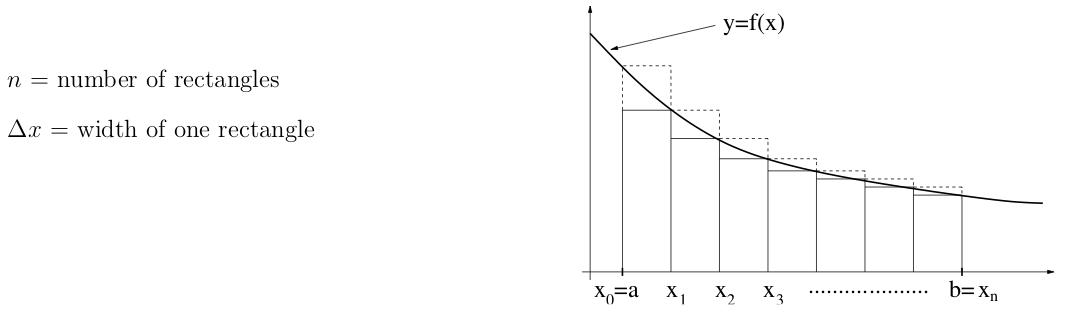
\includegraphics [scale=.75]{5_2_g2}\\

\begin{enumerate}
\item Consider the rectangular approximation of $\displaystyle \int_{1}^{3}\left(0.5x^{2}+\frac{x}{3}\right)\, dx$ shown on the graph.\\

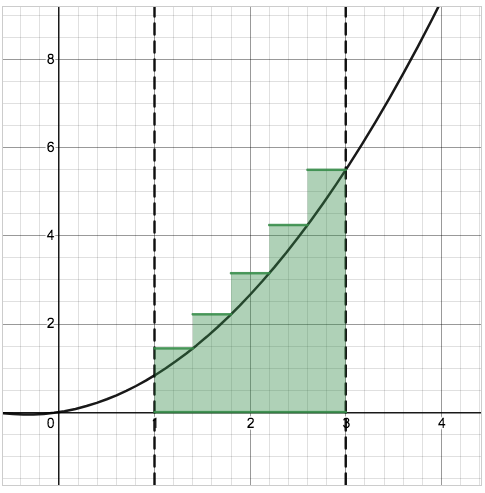
\includegraphics [scale=.35]{5_2_sum2}\\
	\begin{enumerate}
	\item Is this a right or left rectangular approximation?
	\item Is it an under or over approximation of the integral?
	\item Write an expression for the right rectangular approximation using summation notation.
	\vfill
	\end{enumerate}

\newpage

$\hspace{10px}$ \\

\item Let $f$ be the graph of the function shown to below. Calculate each of the integrals that follow exactly.\\
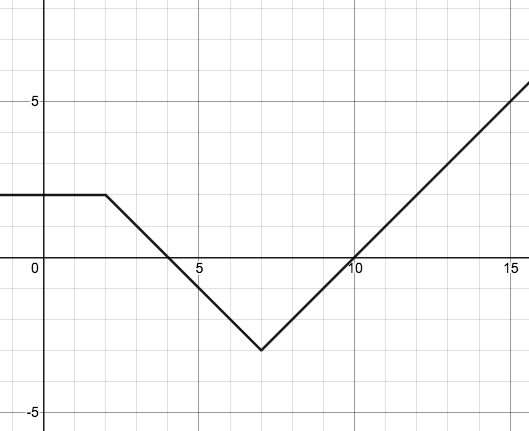
\includegraphics [scale=.35]{5_2_g4}\\
	
	\begin{enumerate}
	\item $\displaystyle \int_0^1f(x)\,dx=$

	\item$\displaystyle \int_0^2f(x)\,dx=$
	\item $\displaystyle \int_0^4f(x)\,dx=$
	\item$\displaystyle \int_4^7f(x)\,dx=$
	\item $\displaystyle \int_0^15f(x)\,dx=$
	\item$\displaystyle \int_7^13f(x)\,dx=$
	\end{enumerate}


\item Let $g$ be the function defined on $0\leq t\leq 20$, some of whose values are shown in the table below.\\
 
\begin{tabular}{c|ccccc}
$t$ & 0 &5  & 10 & 15&20 \\
\hline
$g(t)$ & 30 & 20 &8  &0&-2  \\
\end{tabular}

	\begin{enumerate}
	\item Estimate the value of $\displaystyle \int_0^{12} f(x)\,dx$ using left rectangular sums.\\
	\vfill
	\item Is your estimate an over or under estimate? Why?\\
		\vfill
	\item Find a more accurate estimate of the integral. Why is it more accurate?\\
		\vfill
	\end{enumerate}
\end{enumerate}
\end{document} 

%%%%%%%%%

\item Use a left sum and a right sum, with $n = 4$, to estimate the area under the curve $f(x) = x^2 + 2$ on the interval $0 \leq x \leq 8$.\\
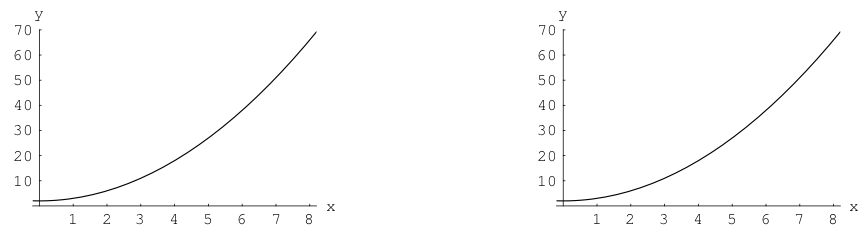
\includegraphics [height=50mm, width=150mm]{5_2_g1}\\
\vfill
\item Describe, in general, a way to find the \textit{exact} area under a curve.\\
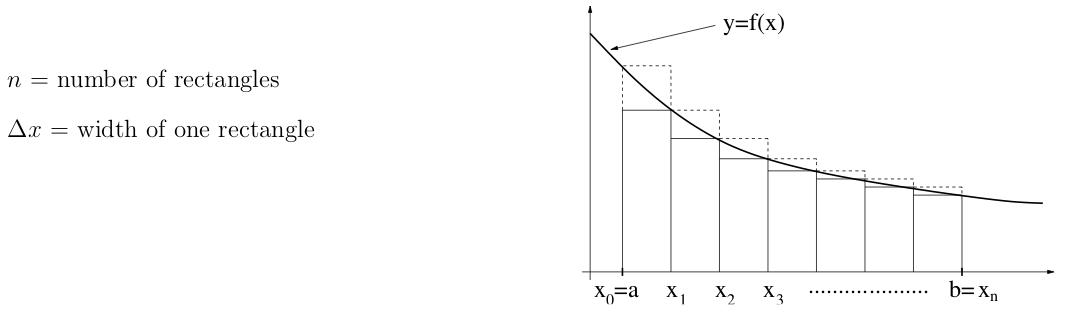
\includegraphics [height=50mm, width=150mm]{5_2_g2}\\
Left Sum =\\
\vfill
Right Sum =\\
\vfill



\begin{tcolorbox}
\textbf{Warm-up: } Solve the following equations for $t$.
\begin{multicols}{2}
\begin{enumerate}
\item $(t+1)^2=9$
\item $tx+x^2=5$
\end{enumerate}
\end{multicols}
\end{tcolorbox}

MINIPAGE
\noindent\begin{minipage}{0.3\textwidth}% adapt widths of minipages to your needs
try 1
\end{minipage}%
\hspace{40mm}
\begin{minipage}{0.6\textwidth}
a) $f'(2)=$\\\

b) $f'(4)=$\\

c) $f'(6)=$\\

d) $f'(7)=$\\

e) $f'(8)=$
\end{minipage}
